
\section{Charge extortion \ddc}
\label{chap5:sect:chargeExtortion}
This section explains the charge extortion mechanism at work during BBI which allows fault creation.
The voltage pulse generator, at each edge of its pulse, injects and then extorts electrical charges into and out of the IC.
%\subsection{Logic considerations \ddc}
%\label{chap5:sect:chargeExtortion:subsect:logicConsiderations}
%
%\begin{figure}[htbp!]
    \centering
    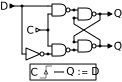
\includegraphics[width=0.6\textwidth]{5_faultModel/figures/dffLogic.pdf}
    \caption{D Flip-Flop logic schematic}
    \label{chap:5;fig:dffLogic}
\end{figure}
%In order to understand electrically why faults occur, it is important to begin with logic considerations.
%Nowadays, the vast majority of commercial ICs are sequential.
%The main building block of a sequential IC is the Edge-Triggered D Flip-Flop (DFF).
%Fig. \ref{chap:5;fig:dffLogic} presents the logic schematic of a DFF.
%Because DFFs work on clock edges, it is interesting to target them at specific times when performing fault injection.
%\textcolor{magenta}{Paragraphe à terminer, compléTer, revoir...}
%%The block has two inputs and two outputs.
%%This building block is ruled by a clock, input at C.
%%At each rising edge of the clock, the output samples the input value.
%%It is thus a memory cell, which stores at Q for a short amount of time the value present at D.
%%What is important to remember here is that outside of the rising edge, any change at D is not seen at Q.
%%Therefore, when performing fault injections, it is interesting to affect the value at D long enough to let the DFF sample an incorrect value.
%This fault model has been proposed in \cite{emfiFF} for EMFI.
%
%\textcolor{magenta}{Parler du fait que les circuits séquentiels échantillonnent périodiquement les valeurs des DFFs (registres). Du coup, si on change un niveau logique suffisamment longtemps pour qu'il perdure pendant l'échantillonnage, c'est gagné ! Faute !, sinon Non.}

\subsection{Sequential logic operation \ddc}
\label{chap5:sect:chargeExtortion:subsect:seqLogic}
Sequential logic is implemented everywhere in modern integrated circuits.
It consists of logic gates fulfilling a function, followed by sample elements, the Edge-Triggered D Flip-Flop (DFF).
DFFs are governed by a clock, and as their name implies, at each rising-edge or falling-edge (depending on the design) of the clock, they sample their input and replicate it on their output.
Therefore, if an attacker manages to disturb the input of one or several DFFs at a specific time, located around the triggering edge, it enables the possibility of inducing faulty behavior in the logic.

\begin{figure}[H]
    \centering
    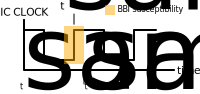
\includegraphics[width=15cm]{5_faultModel/figures/bbiFaultSusceptibility.pdf}
    \caption{BBI sampling fault susceptibility}
    \label{chap:5;fig:bbiSusc}
\end{figure}
Sequential logic basic principle of operation is depicted in Fig. \ref{chap:5;fig:bbiSusc}, alongside a BBI timing susceptibility fault model.
This fault model was first introduced in \cite{emfiFF} for EMFI.
It states that to maximize fault creation with electromagnetic disturbances, the latter have to appear during a specific period of time in order to be successful.

%
%%This fault model has been proposed in \cite{emfiFF} for EMFI.
%
%With the previous fault model in mind, let's have deeper look at it.
%Fig. \ref{chap:5;fig:bbiSusc} presents the sampling fault model we are going to discuss.
%It states that to maximize fault creation, faults have to be injected during a specific period of time.
%It is precisely located before and after every clock rising edge.

\subsection{Charge extortion \ddc}
\label{chap5:sect:chargeExtortion:subsect:chargeExtortion}
